%\documentstyle[epsf,twocolumn]{jarticle}       %LaTeX2e仕様
%\documentclass[twocolumn]{jarticle}     %pLaTeX2e仕様(platex.exeの場合)
\documentclass[onecolumn]{ujarticle}   %pLaTeX2e仕様(uplatex.exeの場合)
%%%%%%%%%%%%%%%%%%%%%%%%%%%%%%%%%%%%%%%%%%%%%%%%%%%%%%%%%%%%%%
%%
%%  基本バージョン
%%
%%%%%%%%%%%%%%%%%%%%%%%%%%%%%%%%%%%%%%%%%%%%%%%%%%%%%%%%%%%%%%%%
\setlength{\topmargin}{-45pt}
%\setlength{\oddsidemargin}{0cm}
\setlength{\oddsidemargin}{-7.5mm}
%\setlength{\evensidemargin}{0cm}
\setlength{\textheight}{24.1cm}
%setlength{\textheight}{25cm}
\setlength{\textwidth}{17.4cm}
%\setlength{\textwidth}{172mm}
\setlength{\columnsep}{11mm}

%\kanjiskip=.07zw plus.5pt minus.5pt


% 【節が変わるごとに (1.1)(1.2) … (2.1)(2.2) と数式番号をつけるとき】
%\makeatletter
%\renewcommand{\theequation}{%
%\thesection.\arabic{equation}} %\@addtoreset{equation}{section}
%\makeatother

%\renewcommand{\arraystretch}{0.95} 行間の設定
%%%%%%%%%%%%%%%%%%%%%%%%%%%%%%%%%%%%%%%%%%%%%%%%%%%%%%%%
%\usepackage{graphicx}   %pLaTeX2e仕様(\documentstyle ->\documentclass)
\usepackage[dvipdfmx]{graphicx}
\usepackage{subcaption}
\usepackage{multirow}
\usepackage{amsmath}
\usepackage{url}
\usepackage{ulem}
%%%%%%%%%%%%%%%%%%%%%%%%%%%%%%%%%%%%%%%%%%%%%%%%%%%%%%%%
\begin{document}

	%bibtex用の設定
	%\bibliographystyle{ujarticle}
	\noindent

	\hspace{1em}
	2019 年 9 月 27 日
	ゼミ資料
	\hfill
	M1 寺内 光

	\vspace{2mm}

	\hrule

	\begin{center}
		{\Large \bf 進捗報告}
	\end{center}


	\hrule
	\vspace{3mm}

	% ‚ここから 文章 Start!
	\section{オーストラリアから帰還}
	ひとまず無事に帰ってきました.初めての国際学会の洗礼を受けました.

	\section{今週やったこと}
	google の official 版 DeepLab v3+ \cite{deeplabv3_official} のサンプルコードをデータセットに PASCAL VOC 2012 \cite{pascal-voc-2012} を用いて動かすことができた.
	表 \ref{tab:class_pascal_voc} にクラスとインデックスを示す.

	\begin{table}[h]
		\centering
		\caption{pascal voc のクラス一覧とインデックス}
		\vspace{-1mm}
		\label{tab:class_pascal_voc}
		\begin{tabular}{|c|c|c|c|} \hline
			Index&Class&Index&Class\\ \hline\hline
			0&background&11&dining table\\ \hline
			1&aeroplane&12&dog\\ \hline
			2&bicycle&13&horse\\ \hline
			3&bird&14&motor bike\\ \hline
			4&boat&15&person\\ \hline
			5&bottle&16&potted plant\\ \hline
			6&bus&17&sheep\\ \hline
			7&car&18&sofa\\ \hline
			8&cat&19&train\\ \hline
			9&chair&20&tv/monitor\\ \hline
			10&cow&(255)&(void)\\ \hline
		\end{tabular}
	\end{table}

	インデックスにあたる部分が PNG 画像のカラーと対応している.つまり,画素値を見ればそれがクラスインデックスになっているらしい.

	図 \ref{fig:prediction1}, \ref{fig:prediction2} に学習済み重みを用いた prediction 結果を示す.

	\begin{figure}[t]
		\centering
		\vspace{-7mm}
		\begin{subfigure}{0.45\columnwidth}
			\centering
			\hspace*{-5mm}
			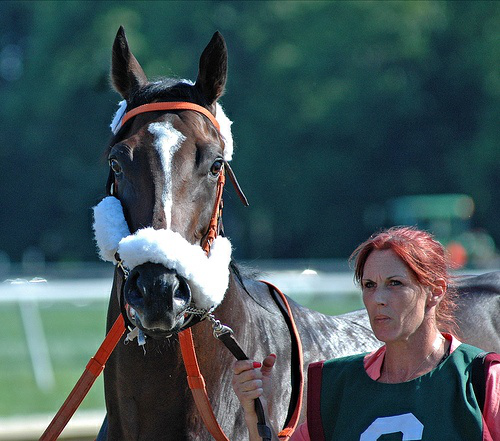
\includegraphics[width=1.3\columnwidth]{000024_image.png}
			\caption{Original}
			\label{fig:original1}
		\end{subfigure}
		\begin{subfigure}{0.45\columnwidth}
			\centering
			\hspace*{-5mm}
			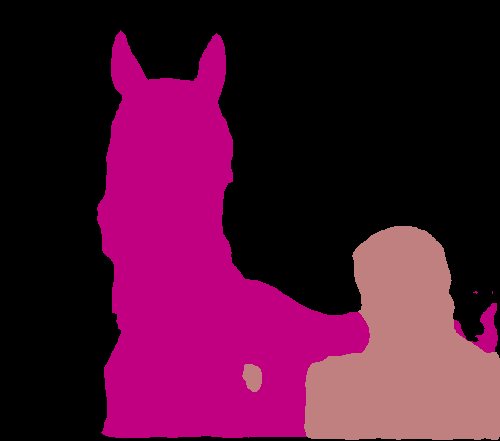
\includegraphics[width=1.3\columnwidth]{000024_prediction.png}
			\caption{Prediction}
			\label{fig:prediction_result1}
		\end{subfigure}
		\caption{prediction結果1}
		\label{fig:prediction1}
	\end{figure}

	\begin{figure}[t]
		\centering
		\vspace{-7mm}
		\begin{subfigure}{0.45\columnwidth}
			\centering
			\hspace*{-5mm}
			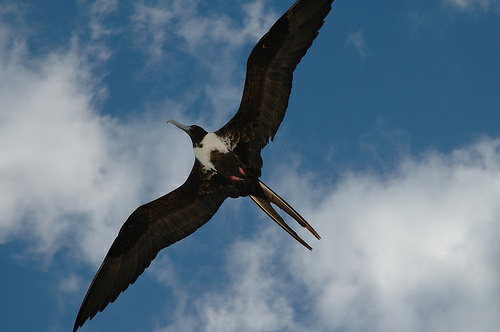
\includegraphics[width=1.3\columnwidth]{000064_image.png}
			\caption{Original}
			\label{fig:original2}
		\end{subfigure}
		\begin{subfigure}{0.45\columnwidth}
			\centering
			\hspace*{-5mm}
			
\includegraphics[width=1.3\columnwidth]{000064_prediction.png}
			\caption{Prediction}
			\label{fig:prediction_result2}
		\end{subfigure}
		\caption{prediction結果2}
		\label{fig:prediction2}
	\end{figure}


	サンプルコードが動かない系のエラーはオーストラリアに行く前にさんざん悩まされた問題だったので一安心.来週は4コマ漫画ストーリーデータセットの形式を Sementic Segmentation で動く形式に整形するところを進めていきたい.

	\section{フロントエンドエンジニア}\noindent
	1研ホームページのブログのフロント開発をしていました.\sout{フロントエンドエンジニアの道が開けたと思います.}

	% 参考文献リスト
	\bibliographystyle{unsrt}
	\bibliography{2019_09_27_terauchi}
\end{document}
